\documentclass[10pt]{article}
\usepackage{NotesTeX} %/Path/to/package should be replaced with package location
\usepackage{lipsum}
\usepackage{tensor}
\usepackage{amsmath,amsthm,amssymb}
\usepackage{hyperref}
\usepackage{physics}
\usepackage{graphicx}
\usepackage{subcaption}
\input{undertilde}


\newcommand{\bs}{\textbackslash}


\title{{\Huge General Relativity}\\{\Large{Class  20 - March 6, 2020}}} %replace with class number
\author{Kevin Rodriguez}

\emailAdd{kevinrodriguez@utexas.edu} %replace with your email
\begin{document}
    \maketitle
    \flushbottom
    \newpage
    \pagestyle{fancynotes}
    %\part{HELLO \LaTeX\,}
	%Use the uncompiled version of this document in itself as a \LaTeX\, style guide for the class you'll be responsible for.
	%While we have spoken of curved spaces throughout the course, we now have enough mathematical tools under our belt to gift the weight of precision to that word. 
	\section{Properties of the Riemann Curvature Tensor}	\label{sec:properties}
    In the last installment of notes, we happily procured the fruit of our labor: the Riemann Curvature Tensor, $\tensor{R}{^\rho_\sigma _\nu _\mu}$, which (as its name would suggest) allows the curvature of a manifold to be specified quantitatively at a point. For reference, we include here the expression for the Riemann tensor as defined in terms of the connection coefficients\footnote{As always in relativity, we choose the connection between tangent spaces of nearby points on the manifold for which the torsion vanishes -- or, equivalently, that for which the connection coefficients are symmetric in their lower indices. To wit: $\Gamma^{\rho}_{[\mu\nu]}=0$.} and their first derivatives:
    \begin{align}
        \tensor{R}{^\rho_\sigma _\nu _\mu} &= \partial_{\mu}\Gamma^{\rho}_{\nu\sigma} - \partial_\nu\Gamma^{\rho}_{\mu\sigma} + \Gamma^{\rho}_{\mu\lambda}\Gamma^{\lambda}_{\nu\sigma} - \Gamma^{\rho}_{\nu\lambda}\Gamma^{\lambda}_{\mu\sigma}	\label{eq:riemann}\\
        &= 2 \partial_{\left[\mu\right.}\Gamma^{\rho}_{\nu\left.\right]\sigma} + 2 \Gamma^{\rho}_{\left[\mu|\lambda|\right.}\Gamma^{\lambda}_{\left.\sigma\right]\nu} . \notag
    \end{align}
    Recalling that the connection coefficients themselves are expressible in terms of a metric and its first derivatives, we see that our intuition from single variable calculus isn't completely obsolete: Understanding curvature once again requires calculating no higher than the second derivatives of the function at hand. However, properties that we once took for granted while navigating our familiar old flat spaces -- such as the fact that vectors remain unchanged after parallel transporting about a closed path, or that parallel geodesics remain so across the manifold -- are no longer strictly true in curved spaces. It is Riemann's tensor that allows us to abstract these notions towards previously unfamiliar spaces so that we may calculate the degree by which geometric objects are distorted by the underlying curvature. \\
    \par As the Riemann tensor is ubiquitous in relativity, it would be worthwhile to familiarize oneself with some of its general properties. The following symmetries are most evident with all indices lowered ($\tensor{R}{_\rho_\sigma_\mu_\nu}=g_{\rho\lambda}\tensor{R}{^\lambda_\sigma_\mu_\nu}$). We list some of these properties here without proof:
    \begin{itemize}
		\item Antisymmetry in the last two indices:	$R_{\rho\sigma \mu \nu} = -R_{\rho\sigma \nu \mu} $.
    \end{itemize}
    This can be seen in expression \eqref{eq:riemann} by simply interchanging $\mu$ and $\nu$. 
    \begin{itemize}
    	\item Antisymmetry in the first two indices:	$R_{\rho\sigma \nu \mu} = -R_{\sigma \rho\mu \nu} $.
    \end{itemize}
    To see this, one must use the symmetry of the metric after multiplying \eqref{eq:riemann} by $g_{\rho\lambda}$ to lower the first index. 
    \begin{itemize}
    	\item Symmetry under pairwise index permutations:	 $R_{\rho\sigma \mu \nu} = R_{\nu \mu \rho\sigma} $.
    \end{itemize}
    As the Riemann tensor is symmetric in both the first two and second two indices independently, we can infer that the expression is invariant under swapping the first and second pairs of indices altogether. These three criteria may be written succinctly as 
    \begin{align}
   		R_{\rho\sigma \left[\mu \nu\right]} = R_{\rho\sigma\mu\nu} = R_{[\rho\sigma]\mu\nu} . \label{eq:pair_symmetries}
   	\end{align}
   	It is also possible to show that, under cyclic permutations of the last three indices, 
   	\begin{align}
    	 R_{\rho\sigma\mu\nu} + R_{\rho\mu\nu\sigma} + R_{\rho\nu\sigma\mu} = 0,
    \end{align}
    or equivalently that there exists the following antisymmetry:
    \begin{itemize}
    	\item Antisymmetry in the last three indices: $R_{\rho\left[\sigma\mu\nu\right]}=0$ .
    \end{itemize}
    The above symmetries lead to a vast reduction in the number of independent components requiring explicit calculation. In $n$ dimensions, the Riemann tensor has $n^4$ components, but it may be shown (see Carroll) that only $n^2 (n^2-1)/12$ of these are independent. For example, in $n=3$ and $n=4$ dimensions, we are left with just $6$ and $20$ independent components, respectively. 

    \section{Bianchi Identity}
    Recall that the Riemann Curvature Tensor may be constructed with our usual torsion-free connection as the commutator of covariant derivatives $\nabla_{\mu}$ acting on an arbitrary vector $V^{\rho}$: 
    \begin{align}
    	\tensor{R}{^\rho_\sigma_\mu_\nu}V^{\sigma} = \left[ \nabla_{\mu}, \nabla_{\nu} \right] V^{\rho} \label{eq:commutator}
    \end{align}
    If we act from the right on both sides of the equation above with yet another covariant derivative, we end up with the following:
    \begin{align}
    	\nabla_{\left[\lambda\right.}R_{\left.\rho\sigma\right]\mu\nu} \sim [[\nabla_{\lambda}, \nabla_{\rho}], \nabla_{\sigma}] + [[\nabla_{\rho}, \nabla_{\sigma}], \nabla_{\lambda}] + [[\nabla_{\sigma}, \nabla_{\lambda}], \nabla_{\rho}] = 0, \label{eq:bianchi}
    \end{align}
    where we have thrown away the arbitrary vector $V^{\rho}$ and used the Jacobi Identity in identifying the sum of cyclically permuted nested commutators as zero. The relation $\nabla_{\left[\lambda\right.}R_{\left.\rho\sigma\right]\mu\nu}=0$ is called the \textbf{Bianchi Identity}.\footnote{While some authors indicate multiple different Bianchi Identities, Carroll simply refers to \eqref{eq:bianchi} as \textit{the} Bianchi Identity.}

    \section{De-constructing the Riemann Tensor} \label{sec:deconstructing}
    In Section \ref{sec:properties} we made significant headway in narrowing our focus towards the elements of the Riemann tensor that contain useful information regarding the curvature of the manifold while minimizing redundant information. For our most important case of interest, $n=4$ dimensions, we were able to use symmetries to ascertain that only $20$ of the $4^4=256$ components were independent degrees of freedom. One might wonder: Can we go further in reducing the Riemann tensor into a simpler form that is still physically meaningful? The answer is: yes!
    \subsection{Ricci Tensor and Ricci Scalar}
    A contraction of the first and third indices of $\tensor{R}{^\rho_\sigma_\mu_\nu}$ gives rise to the \textbf{Ricci tensor}:
    \begin{align}
    	\tensor{R}{^\alpha_\mu_\alpha_\nu} = R_{\mu\nu}	\label{eq:ricci_tensor} .
    \end{align}
    There is no problem of ambiguity in using the symbol $R$ to designate both the Riemann and Ricci tensors, as each will always have either $4$ or $2$ indices, respectively. As a byproduct of the highly symmetric Riemann tensor, the Ricci tensor inherits a symmetry of its own:
    \begin{align}
    	 R_{\mu\nu} = R_{\nu\mu} \notag. 
    \end{align}
    As a rank 2 symmetric tensor, only $10$ of the components of the Ricci tensor are independent. We may even dare to go further. By taking the trace of the Ricci tensor, we form the \textbf{Ricci scalar}:
    \begin{align}
    	 g^{\mu\nu}R_{\mu\nu} = \tensor{R}{^\mu_\mu} = R \label{eq:ricci_scalar} . 
    \end{align}
    These two objects are undoubtedly much simpler than the full Riemann tensor, but in defining them through successive contractions we have necessarily thrown out some of the Riemann tensor's other useful information. That other information is that which is traceless. We can collect this discarded information into another object called the \textbf{Weyl tensor}.
    \subsection{Weyl Tensor}
    In terms of the Riemann tensor, the Ricci tensor and scalar, and the metric, the Weyl tensor is expressed as 
    \begin{align}
    	C_{\rho\sigma\mu\nu} = R_{\rho\sigma\mu\nu} - \frac{2}{(n-2)} \Big( g_{\rho\left[\mu\right.}R_{\left.\nu\right]\sigma} - g_{\sigma\left[\mu\right.}R_{\left.\nu\right]\rho} \Big) + \frac{2}{(n-1)(n-2)} g_{\rho\left[\mu\right.}g_{\left.\nu\right]\sigma} R \label{eq:weyl} . 
    \end{align}
    The above expression, while long-winded, is easy to understand qualitatively. We have merely taken the Riemann tensor and removed all of the information obtainable through self-contractions. As such, it obeys all of the symmetries of the Riemann tensor discussed in Section \ref{sec:properties}. \\
    \par A few subtleties are worth mentioning. For $n=1$ and $n=2$, the Weyl tensor is undefined, and for $n=3$, the Weyl tensor is zero everywhere. Why is this this important? What does is mean physically?\\
    \par First a small aside and a peek ahead: The Ricci tensor is generated directly by matter fields such as the baryonic matter we are comprised of, the dark matter of which we are not, massless fields like the photon, and even the mysterious dark energy. The Weyl tensor, by contrast, describes the so-called \textbf{vacuum curvature} in regions devoid of matter. The Weyl tensor may seem at first limited in scope, but recall for a moment the enormous array of problems in classical electrodynamics which amount to essentially solving Poisson's equation for the electromagnetic potentials in regions which contained no sources at all. These problems can still become enormously complicated, and more importantly, the solutions of such cases describe the transmission of electromagnetic waves through the vacuum.\\
    \par Translating back to general relativity, we see analogously that the Weyl tensor is the object of interest if we are to understand curvature outside of compact objects such as black holes (e.g. Schwarzchild's metric) and the propagation of gravitational waves. In less than $n=4$ dimensional spacetime, it is found that there are not sufficient degrees of freedom available for gravitational waves to propagate at all. This is reflected in the Weyl tensor being identically zero for $n=3$. \\
    \par Another property of the Weyl tensor is that it is \textit{conformal}. A conformal transformation of the metric is one which scales the entire metric tensor by a single scalar function. By claiming that the Weyl tensor is conformal, we mean to say that under such a transformation to the metric tensor, the Weyl tensor remains unchanged. In symbols, we can express this idea as\sn{The brackets indicate that the Weyl tensor is being considered as a functional of the metric.}
   \begin{align}
    	\tensor{C}{^\rho_\sigma_\mu_\nu}[g_{\alpha\beta}] = \tensor{C}{^\rho_\sigma_\mu_\nu}[\Omega^2(x^\gamma)g_{\alpha\beta}] . \notag
    \end{align}
     For this reason, the Weyl tensor is sometimes called the \textbf{conformal tensor}. Alternative theories of gravity often probe the question of why only the Weyl tensor enjoys this property while the Ricci tensor does not. 

    \subsection{Einstein Tensor}
    Upon contracting two pairs indices in the Bianchi Identity \eqref{eq:bianchi}, we come across another geometric object of interest. First expand the Bianchi Identity:
    \begin{align}
    	\nabla_{\left[\lambda\right.}R_{\left.\rho\sigma\right]\mu\nu} = \frac{2}{3!}\Big( \nabla_{\lambda}R_{\rho\sigma\mu\nu} + \nabla_{\rho}R_{\sigma\lambda\mu\nu} + \nabla_{\sigma}R_{\lambda\rho\mu\nu} \Big) = 0, \notag
    \end{align}
    where we have used the antisymmetry of the Riemann tensor in the last two indices to collect like terms. Then hit the expression with two factors of the metric to contract twice:
    \begin{align}
    	\Big( g^{\lambda\mu}g^{\sigma\nu} \Rightarrow \nabla_{\left[\lambda\right.}R_{\left.\rho\sigma\right]\mu\nu} \Big) \Longrightarrow g^{\lambda\mu} \nabla_{\lambda}\tensor{R}{_\rho^\nu_\mu_\nu} + g^{\lambda\mu} \nabla_{\rho}\tensor{R}{^\nu_\lambda_\mu_\nu} + g^{\sigma\nu}\nabla_{\sigma}\tensor{R}{^\mu_\rho_\mu_\nu} = 0 . \notag
    \end{align}
    We can simplify by making use of our expressions for the Ricci tensor and Ricci scalar.
   	\begin{align}
    	 g^{\lambda\mu} \nabla_{\lambda}\tensor{R}{_\rho_\mu} - \nabla_{\rho}R + g^{\sigma\nu}\nabla_{\sigma}\tensor{R}{_\rho_\nu} = 0 . \notag
    \end{align}
    The first and last terms are identical, dummy indices aside, so we may add them:
   	\begin{align}
    	2 g^{\lambda\mu} \nabla_{\lambda}\tensor{R}{_\rho_\mu} - \nabla_{\rho}R  = 0 . \notag
    \end{align}
    Lastly, if we write $\nabla_{\rho}=\delta^{\lambda}_{\rho}\nabla_{\lambda}=g^{\lambda\mu}\nabla_{\lambda}g_{\mu\rho}$, we can pull out a common covariant derivative\sn{Remember that under the Christoffel connection, the covariant derivative commutes with the metric tensor. This property is called \textbf{metric compatibility}.}:
    \begin{align}
    	 2g^{\lambda\mu} \nabla_{\lambda} \underbrace{\left( \tensor{R}{_\mu_\rho} - \frac{1}{2}g_{\mu\rho}R \right)}_\text{\large $G_{\mu\rho}$}  = 0 . \notag
    \end{align}
    The quantity in brackets denoted $G_{\mu\rho}$ is called the \textbf{Einstein tensor} and according to our expression above, it is a conserved quantity under covariant differentiation. What does it mean for this special combination of curvature measures to be conserved? We may consider this mathematical expression as foreshadowing for the time being. Perhaps we could find a way to relate this $G_{\mu\nu}$ to another conserved quantity that is expressible as a rank 2 symmetric tensor...

    \section{Subtleties Regarding Curvature}
    It is important to note that the Riemann curvature tensor informs us only of the \textit{intrinsic} curvature of the manifold. To better understand this, consider the familiar example of an ellipsoid, which we often visualize as being a two dimensional surface embedded in a three dimensional space. Our combinatorics tell us that, for $n=2$, only $2^2 (2^2-1) / 12=1$ number is required to describe the curvature of the ellipsoid. Common sense says otherwise -- clearly two numbers are necessary! This is because we are appealing to our ability to embed the object in a higher dimensional space to examine its \textit{extrinsic} curvature. For all intents and purposes, the Riemann tensor is only capable of informing us of the intrinsic curvature without recourse to embedding in higher dimensions, and we restrict our interest for the moment to intrinsic curvature alone while reminding ourselves not to let everyday intuition lead us astray. 

    \section{Introduction to Geodesic Deviation}
    One measurable manifestation of curvature on a manifold is the fact that initially parallel geodesics may not remain parallel on the entirety of the manifold. With regards to massive test particles falling freely on a curved spacetime, we observe this quite readily in our favorite thought experiment: Two inertial observers in outer space falling freely towards Earth will notice their relative distance of separation to shrink as they advance towards their home. We now have the mathematical machinery to calculate the deviations amongst neighboring geodesics as they sprawl across the manifold. This is also a first step towards connecting our knowledge of curvature to traditional Newtonian gravity. \\

    \par We need a system to identify which geodesic(s) we want to focus on, and how far along each geodesic we are. These two numbers, which we will call $s$ and $t$, will suffice to define every point on the manifold. If each geodesic $s$ has coordinates $x_{(s)}^{\mu}(t)$, with $t$ an affine parameter on the curve, then we may similarly assign a tangent vector $T_{(s)}^{\mu} = dx_{(s)}^{\mu}/dt$ to each geodesic. 

    \begin{figure}[h!]
	\centering
	\tikzset{every picture/.style={line width=0.75pt}} %set default line width to 0.75pt        
	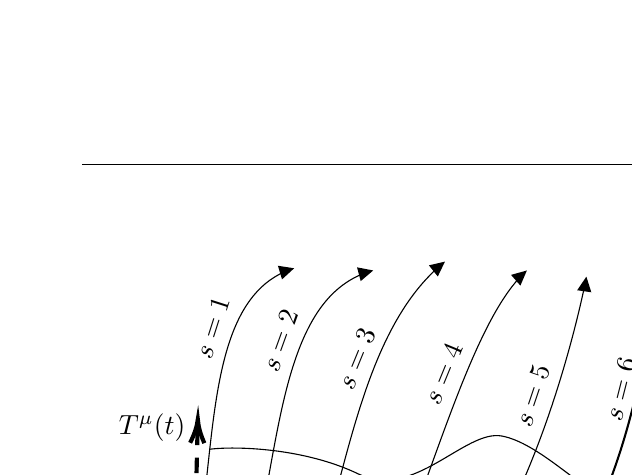
\begin{tikzpicture}[x=0.75pt,y=0.75pt,yscale=-0.8,xscale=0.8]
	%uncomment if require: \path (0,300); %set diagram left start at 0, and has height of 300

	%Curve Lines [id:da7466653756911263] 
	\draw    (148.22,248.72) .. controls (209.33,209.28) and (164.42,41.4) .. (237.27,15.72) ;
	\draw [shift={(239.52,14.99)}, rotate = 523.1600000000001] [fill={rgb, 255:red, 0; green, 0; blue, 0 }  ][line width=0.08]  [draw opacity=0] (8.93,-4.29) -- (0,0) -- (8.93,4.29) -- cycle    ;
	%Curve Lines [id:da1549633009163982] 
	\draw    (179.5,248) .. controls (240.61,208.56) and (209.16,40.39) .. (284.8,16.97) ;
	\draw [shift={(287.13,16.31)}, rotate = 525.27] [fill={rgb, 255:red, 0; green, 0; blue, 0 }  ][line width=0.08]  [draw opacity=0] (8.93,-4.29) -- (0,0) -- (8.93,4.29) -- cycle    ;
	%Curve Lines [id:da009075382666697607] 
	\draw    (207.5,248) .. controls (271.66,236.18) and (256.81,73.3) .. (328.14,12.81) ;
	\draw [shift={(330.33,11)}, rotate = 501.37] [fill={rgb, 255:red, 0; green, 0; blue, 0 }  ][line width=0.08]  [draw opacity=0] (8.93,-4.29) -- (0,0) -- (8.93,4.29) -- cycle    ;
	%Curve Lines [id:da03715950821689562] 
	\draw    (254.66,247.41) .. controls (300.25,252.65) and (330.16,64.59) .. (377.5,18.34) ;
	\draw [shift={(379.67,16.33)}, rotate = 498.84] [fill={rgb, 255:red, 0; green, 0; blue, 0 }  ][line width=0.08]  [draw opacity=0] (8.93,-4.29) -- (0,0) -- (8.93,4.29) -- cycle    ;
	%Curve Lines [id:da9682412073509172] 
	\draw    (296.5,247) .. controls (373.99,209.2) and (410.4,46.38) .. (415.02,22.67) ;
	\draw [shift={(415.5,20)}, rotate = 458.13] [fill={rgb, 255:red, 0; green, 0; blue, 0 }  ][line width=0.08]  [draw opacity=0] (8.93,-4.29) -- (0,0) -- (8.93,4.29) -- cycle    ;
	%Curve Lines [id:da49004009378226354] 
	\draw [line width=0.75]    (333.37,246.1) .. controls (430.99,223.37) and (450.91,69.71) .. (458.07,19.87) ;
	\draw [shift={(458.39,17.67)}, rotate = 458.28] [fill={rgb, 255:red, 0; green, 0; blue, 0 }  ][line width=0.08]  [draw opacity=0] (8.93,-4.29) -- (0,0) -- (8.93,4.29) -- cycle    ;
	%Straight Lines [id:da19346279268684263] 
	\draw [line width=1.5]    (394.51,209.21) -- (441,151.12) ;
	\draw [shift={(443.5,148)}, rotate = 488.67] [fill={rgb, 255:red, 0; green, 0; blue, 0 }  ][line width=0.08]  [draw opacity=0] (11.61,-5.58) -- (0,0) -- (11.61,5.58) -- cycle    ;
	\draw [shift={(394.51,209.21)}, rotate = 308.67] [color={rgb, 255:red, 0; green, 0; blue, 0 }  ][fill={rgb, 255:red, 0; green, 0; blue, 0 }  ][line width=1.5]      (0, 0) circle [x radius= 4.36, y radius= 4.36]   ;
	%Curve Lines [id:da7809418091783804] 
	\draw    (179.5,189) .. controls (194.57,187.04) and (232.5,192) .. (269.5,204) .. controls (306.5,216) and (331.5,185) .. (353.5,189) .. controls (375.5,193) and (382.5,206) .. (394.5,209) ;
	%Curve Lines [id:da582328329140043] 
	\draw    (186.5,156) .. controls (201.57,154.04) and (239.5,159) .. (276.5,171) .. controls (313.5,183) and (340.5,148) .. (362.5,152) .. controls (384.5,156) and (398.5,183) .. (410.5,186) ;
	%Curve Lines [id:da8893456443463101] 
	\draw    (188.5,124) .. controls (203.57,122.04) and (245.5,123) .. (278.5,139) .. controls (311.5,155) and (342.5,112) .. (364.5,116) .. controls (386.5,120) and (413.5,149) .. (425.5,152) ;
	%Curve Lines [id:da9921558105586963] 
	\draw    (171.5,220) .. controls (186.57,218.04) and (224.5,223) .. (261.5,235) .. controls (298.5,247) and (305.5,221) .. (327.5,225) .. controls (349.5,229) and (346.5,235) .. (358.5,238) ;
	%Straight Lines [id:da7901541842541708] 
	\draw [line width=1.5]    (397.04,211.19) -- (435.47,244.39) ;
	\draw [shift={(438.5,247)}, rotate = 220.82] [fill={rgb, 255:red, 0; green, 0; blue, 0 }  ][line width=0.08]  [draw opacity=0] (11.61,-5.58) -- (0,0) -- (11.61,5.58) -- cycle    ;
	\draw [shift={(394.5,209)}, rotate = 40.82] [color={rgb, 255:red, 0; green, 0; blue, 0 }  ][line width=1.5]      (0, 0) circle [x radius= 4.36, y radius= 4.36]   ;
	%Shape: Square [id:dp6136088637535175] 
	\draw   (401.44,201.24) -- (409.41,208.17) -- (402.48,216.14) -- (394.51,209.21) -- cycle ;
	%Straight Lines [id:da8190340897072039] 
	\draw [line width=1.5]  [dash pattern={on 5.63pt off 4.5pt}]  (179.5,189) -- (181.43,109) ;
	\draw [shift={(181.5,106)}, rotate = 451.38] [color={rgb, 255:red, 0; green, 0; blue, 0 }  ][line width=1.5]    (14.21,-4.28) .. controls (9.04,-1.82) and (4.3,-0.39) .. (0,0) .. controls (4.3,0.39) and (9.04,1.82) .. (14.21,4.28)   ;
	\draw [shift={(179.5,189)}, rotate = 271.38] [color={rgb, 255:red, 0; green, 0; blue, 0 }  ][fill={rgb, 255:red, 0; green, 0; blue, 0 }  ][line width=1.5]      (0, 0) circle [x radius= 4.36, y radius= 4.36]   ;

	% Text Node
	\draw (460.99,160.03) node  [rotate=-1.31]  {$\boldsymbol{\vec{\partial }_{t}}$};
	% Text Node
	\draw (190.31,50.71) node  [rotate=-287.7]  {$s=1$};
	% Text Node
	\draw (231.31,58.71) node  [rotate=-289.85]  {$s=2$};
	% Text Node
	\draw (277.31,69.71) node  [rotate=-292.35]  {$s=3$};
	% Text Node
	\draw (329.31,78.71) node  [rotate=-292.35]  {$s=4$};
	% Text Node
	\draw (383.31,91.71) node  [rotate=-288.62]  {$s=5$};
	% Text Node
	\draw (436.31,87.71) node  [rotate=-284.3]  {$s=6$};
	% Text Node
	\draw (418.99,248.03) node  [rotate=-1.31]  {$\boldsymbol{\vec{\partial }_{s}}$};
	% Text Node
	\draw (154,111) node    {$T^{\mu }( t)$};
	% Text Node
	\draw (153,196) node    {$x^{\mu }( t)$};
	\end{tikzpicture}
	\caption{A family of geodesics labeled by $s$ and parameterized by $t$.}
	\end{figure}

	\par To construct an orthogonal coordinate system, we take our tangent vectors to be basis vectors $\vec{T}=\vec{\partial_t}$ and require that they be perpendicular to $\vec{S}=\vec{\partial_s}$ everywhere such that $T^{\mu}S_{\mu}=0$. The relative velocity can be defined as 
	\begin{align}
		V^{\nu}=S^{\mu}\nabla_{\mu}T^{\nu}. \notag
	\end{align}
	The acceleration similarly is defined as
	\begin{align}
		A^{\rho}=S^{\mu}\nabla_{\mu}(S^{\nu}\nabla_{\nu}T^{\rho})=S^{\mu}\nabla_{\mu}V^{\rho}. \notag
	\end{align}
	The necessary calculation will be covered in the next set of notes, but the punchline is 
	\begin{align}
		A^{\mu}=\tensor{R}{^\mu_\nu_\rho_\sigma}T^{\nu}T^{\rho}S^{\sigma}.
	\end{align}
	This equation is called the \textbf{geodesic deviation equation}. It tells us precisely how neighboring geodesics are drawn towards or away from each other in terms of the Riemann curvature tensor. 

%%%%%%%%%%%%%%%%%%%%%%%%%%%%%%%%%%%%%%%%%%
\end{document}

